\section{Application Development}
This chapter provides a complete rundown on the development process of the fake news detection application build for this thesis, from inception to completion.

\subsection{Functionalities}
  The application developed for this thesis is a web extension built for Google Chrome, which provides users with an accessible tool for evaluating the reliability of online news. The extension performs a multifaceted analysis of any given news article, based upon its URL, headline, content and authors, by means of machine learning algorithms, web scraping and crowdsourcing.

  The key functionalities of the application are the following:
  \begin{enumerate}
    \item upon landing on an online news article from a known news source, automatically extract some critical information about the article, based on its HTML source code (i.e. URL, headline, content and authors)
    \item after successfully extracting the required information about the article, automatically initiate a multifaceted reliability analysis, which rates the current article from the following standpoints:
    \begin{enumerate}
      \item the biased/deceptive character of the language used in the content of the article, predicted by one of the machine learning algorithms implemented for content-based fake news detection
      \item the deceptive/sensationalist character of the language used in the headline of the article, predicted by one of the machine learning algorithm implemented for title-based clickbait detection
      \item the reliability of the source based upon the list of reliable / perennial sources web-scraped from Wikipedia \cite{wiki_reliable_sources}
      \item the reliability of the source based upon previous user feedback
      \item the credibility of the authors based upon previous user feedback
    \end{enumerate}
    \item after the completion of the analysis, the users have the ability to provide their own rating / feedback for the article
  \end{enumerate}

\subsection{Architecture and Technologies}

\begin{figure}[h]
  \centering
  \fbox{\includegraphics[width=0.8\textwidth,keepaspectratio]{images/app-architecture.png}}
  \caption{Diagram depicting the architecture of the application.}
\end{figure}
  
\subsubsection{Front-end}
  The \textbf{client-side} (\textbf{front-end}) of the application was built as a Chrome Extension, so that all the fake news detection and reliability analysis functionalities are immediately accessible upon opening a given news article on the browser. Compared to a standard web front-end application, a Chrome extension (and browser extensions in general) have a more peculiar architecture. 

  Chrome extensions have three main components:
  \begin{enumerate}
    \item \textbf{Service Worker}, a JavaScript script running in the background of the browser, reacting to events emitted from the browser, such as tabs/windows being open/closed, refreshing the webpage, modifying the URL from a tab etc. Compared to popup and content scripts, the lifecycle of the service worker is not dependent of any webpage. Therefore, the service worker can be running across webpages, terminate only after becoming idle and restart only when needed (i.e. when having to handle an event from the browser). Service workers are also useful if one wants to store a temporary local state shared across tabs or run an action in the background which should not run only while the popup of the extension is open.
    \item \textbf{Popup}, the user interface of the chrome extension, which gets toggled when clicking on the icon of the extension located on the taskbar. By means of HTML, CSS and JavaScript, an interface comparable to an ordinary webpage can be written, with certain implicit limitations, such as lack of routing, cannot use standard Redux for state management etc. The lifecycle of the popup lasts only while the popup is open, so if one wants to preserve state between popup sessions, one should either choose to store state in the background script, localStorage or Chrome's Sync or Local Storage.
    \item \textbf{Content Script}, JavaScript scripts running in the context of webpages. They are useful when it comes to reading or modifying the Document Object Model (DOM) of the webpage. Even though they can perform changes to the HTML and CSS source code of the webpage, they are unable to interact with the JavaScript of the webpage (i.e. access and use functions or variables defined in the context of the web page or extension). Also, they cannot access the Chrome APIs and events. Despite having these limitations, which many have as workaround to communicate via a messages protocol with parent extension, content scripts are useful in many scenarios.
  \end{enumerate}

  The popup of the news reliability extension was written using the JavaScript library called React, which provides a more efficient development environment and functionalities for writing component-based web interfaces. With the help of components, different logical parts of the view can be separated by concerns.

  As for the programming language, I used TypeScript instead of simple JavaScript. TypeScript is a strongly-typed superset of JavaScript, which enables writing code less prone to errors, thanks to the introduction of static typing. 

  As for the programming paradigm, the code written can be mostly categorized as functional and procedural. Classes were used at minimum, and all the user interface components, service functions, utility functions, React hooks were writing as functions, attempting to respect some of basic functional programming principles: immutable state, no side effects (as much as possible), functions as first-class entities, some use of pure functions and type systems.

  \begin{figure}[h]
    \centering
    \fbox{\includegraphics[width=0.8\textwidth,keepaspectratio]{images/react-components.jpeg}}
    \caption{Component-based structure of the user interface.}
  \end{figure}
  
  For styling, instead of plain CSS, TailwindCSS was used instead. TailwindCSS (i.e. similar to Bootstrap, but more customizable), is essentially a large collection of customizable CSS classes, which eliminates the need of having separate CSS files and all the styling can be done by adding the needed classes to the HTML elements.

  For HTTP requests to the RESTful APIs build on the back-end, the Axios library was chosen. Axios facilitates the process of creating asynchronous requests. 

\subsubsection{UI Design}
  Prior to coding the user interface, I followed the good practice of creating design mockups first. Design mockups are of great utility to pre-plan and visualize how the UI elements should be organized in order to not only have a clean and attractive appearance, but to also project and create the best workflow for the application. For this purpose, I made use of Adobe's UI/UX design software called Adobe XD, which was also useful for creating some graphical elements, such as logos, icons and buttons designs.

  \begin{figure}[h]
    \centering
    \fbox{\includegraphics[width=0.8\textwidth,keepaspectratio]{images/design-mockup.png}}
    \caption{Design mockup of some of the pages and graphical elements.}
  \end{figure}

\subsubsection{Back-end}
  On the server-side (back-end), two servers (RESTful APIs) were built. On the one hand, a server was required to train and expose the machine learning models built for article content-based and headline-based fake news detection. On the other hand, another server was needed to manage some persistent state of the application, such as the set of news sources which are automatically recognized by the web extension or the history of user feedbacks/ratings submitted.

  First of all, the server for the machine learning algorithms was built using Python. Python is probably the most popular choice for machine learning, because of its simplicity, flexibility and solid libraries and frameworks.

  Scikit-learn is one of the essential libraries used withing this project. It is one of the most popular machine learning algorithms, which provides access to a great variety of machine learning classification and regression algorithms, including all those used in this application: k-nearest neighbor, decision tree, logistic regression and support vector machine. Furthermore, Scikit-learn also gives access to various Natural Language Processing related tools, such as the TF and TF-IDF feature extraction methods which where applied during the training process of the models.
  
  In addition to Skicit-learn, another natural language processing library which came in handy during the development of the classifiers was NLTK (Natural Language Toolkit). This library was primarily used in the pre-processing phase of the each training sessions. NLTK provided tool for each required pre-processing operation, namely tokenizations, lemmatization, stemming, removal of punctuation and removal of stop words.

  In machine learning, advanced data manipulation is a fundamental task necessary for by and large every algorithm. In this project, Pandas was leveraged for this purpose. Pandas was particularly useful in loading the datasets stored into CSV file and apply all the data pre-processing and data leakages cleaning.

  Partially, the machine learning models that were trained are exposed to the Chrome extension via a RESTful API built using Flask. Flask is a framework for creating python APIs and it often regarded as a microframework, because it does not require any libraries or tools. 

  A secondary purpose the python server fulfills, besides the machine learning tasks, is an API which receiving as query parameter the URL to a  webpage (specifically, to a news article), responds with some attributes of the website later used for the reliability analysis (i.e. content, headline and authors). In order to do this, the Newspaper python tool was used, which via some complex algorithms, several of them involving AI, can extract with a decent performance the aforementioned attributes. Initially, I attempted to extract these attributes manually, with no additional library, by merging all the p HTML tags to retrieve the content, take the heading HTML attribute for the title and look after elements with a class name containing the words "author" or "contributors" to get the authors. Nonetheless, achieving this task proven more difficult than originally anticipated, due to the manifold variables that appear in the HTML structure of each different website.

  As for the programming paradigm, opposite to the procedural and functional style adopted at the front-end level, the Python application is based on the Object-Oriented Programming principles, such as abstraction, encapsulation or polymorphism. The classes for the first of the machine learning models were designed and written so that they could be re-used and adapted to other machine learning tools with a minimal number of modifications. This facilitated an accessible iteration through various algorithms, feature extraction methods and datasets, both for content-based and headline-based fake news detection methods.

  Second of all, the API built for managing the server state of the application, such as the news sources scraped, previous reliability analysis and user ratings, was developed using Node.js, with the Express framework. Node.js and Express were chosen for the outstanding flexibility and freedom in architectural preferences, the multitudinous libraries and NPM (Node Package Manager) packages. Moreover, using the same language both on the front-end and the back-end (i.e. TypeScript), comes as a benefit when having to couple them together. 

  Besides managing the data of the application via CRUD operations, the Node.js server was also responsible with the web-scraping part (i.e. scraping the list of articles classified by their reliability from here \cite{wiki_reliable_sources}). For this purpose, the Cheerio NPM package was used, which provides a tool for retrieving and parsing the DOM of any webpage given its URL.

\subsubsection{Database}
  The server is connected to a NoSQL database, created by means of MongoDB, which is JSON-like document oriented cross-platform database management program. If in case of SQL entities are represented as tables, in MongoDB each entity is a document. MongoDB is a popular choice for modern applications thanks to its high performance levels (storing most of the data into the RAM), speed and availability (performs tens of times faster than relational databases), flexibility (does not have a pre-defined schema, offering a dynamic schematic architecture that works with non-structured data) and scalability.
    
  MongoDB also has some disadvantages, but they bore out not to be prominent during the development of the application: no support for JOIN statements (given its non-relational structure), a limited size of 16MB per document and no support for transactions. 

  To ensure the portability of the application, I decided upon deploying the database to the cloud. I took advantage of the free option provided by MongoDB Atlas. By deploying the server to MongoDB Atlas: a reliable security is ensured for the data, the management of the database is most efficient, there is no need to set up the database locally and the database is practically already prepared for a future production version of the application.

\subsubsection{Testing}
  During the development of the application, both automated and manual testing methods were applied. Automated tests were written predominantly while working on the machine learning algorithms for fake news detection, whereas the front-end of the Chrome extension and the Node.js server managing the state of the application and the web-scraping where mostly tested manually.

  Firstly, the reason for writing automated tested for the machine learning algorithms was to ensure that any changes performed to their logic would not lead to underlying errors that would have negatively affect or result in misleading measures of the actual performance of the models. Practically, this was the most sensitive and error-prone part of the project, so automated test were considered a useful addition.

  Using the unittest Python library for writing test cases, the dataset cleaning, pre-processing and processing methods were tested. Feeding the correct data optimally processed to the model for training is essential and given that changes were often performed to this part of the code to adapt for each task, test prove to be indeed beneficial in detecting errors. Both the test-last and test-first techniques were employed. As highlighted in various studies like \cite{a9}.

  To test the performance of each of the machine learning model, various standard metrics were applied (i.e. accuracy, recall, precision, F1 score).  These techniques are further detailed in the following sections of the thesis.

  For the manual testing of the APIs, I used an API client application called Insomnia, which enabled verifying and validating every API method. Lastly, the front-end was tested by iterating over various scenarios and edge cases through the user interface.

\subsubsection{Management}

For source control management, git was used together with Github. The master branch was used for stable production-ready code, while the development branch was periodically merged into master and used as the base branch in which feature branches were merged. Each feature branch was created for different functionalities and logical parts of the application, to avoid modifying directly stable parts of the code. In case there were some severe bugs to be solved immediately, hotfix branches would be used.

For features and bugs management, given that this was an individual project, I decided on employing a simple tool, without too many complex unneeded functionalities. I used Notion, which enables the creation of Kanban boards, frequently used at industrial-level as well. A Kanban board is split into multiple columns, each of them representing different stages of the development of a feature. Feature ideas would be placed into the "Backlog" column, features that are planned to be implemented in the "Approved Backlog" column, features that are currently in progress into the "Working" column, feature which need to be tested and reviewed further in the "Test/Review" column, features that are completed in the "Done" column and various bugs and improvement ideas were placed into the Bugs/Improvements column. In many of the tickets from the board, I added a description and a checklist of tasks that need to be fulfilled to consider the feature implemented and ready to be moved to the "Test/Review" or the "Finished" column.

\begin{figure}[h]
  \centering
  \fbox{\includegraphics[width=0.8\textwidth,keepaspectratio]{images/notion.png}}
  \caption{Notion Kanban board for features and bugs management.}
\end{figure}

\subsection{Machine Learning Algorithms}
In this section, an outline of the content-based and headline-based fake news detection algorithms is presented, talking about the dataset selection, data processing, feature extraction, training and results.

\begin{figure}[h]
  \centering
  \fbox{\includegraphics[width=0.8\textwidth,keepaspectratio]{images/ml-schema.png}}
  \caption{The process of building a classifier.}
\end{figure}

\subsubsection{Datasets}
For the content-based fake news classification, a dataset \cite{dataset_content} with over 35.000 news articles was chosen, with roughly half of them classified as fake and half of them real. On the one hand, the real news were collected from Reuters articles mostly \cite{a1}, which along with the Associated-Press and Agence France-Presse is one of largest and most generally reliable news agencies in the world. Reuters is known for the objective manner in which the articles are written, hence it can be regarded as a good source to form a dataset of real news. On the other hand, the fake news data is a selection of news classified by PolitiFact and Facebook as fake. PolitiFact is a fact-checking nonprofit project, where journalists, editors and reporters rate articles and claim from politicians. 

However, the dataset is not perfect in its initial form, due to the data leakages it contains \cite{data_leaks}. In the context of machine learning, data or information leakages refer to additional or abnormally distributed information in the training dataset, which can cause misleading model predictions in production. This kind of information is too peculiar to the dataset and does not generally behave the same way for real-life inputs, leading to overfitting. The result is that the machine learning models yield misleadingly high accuracy scores. In order to resolve this issue, the detected data leakages had to be cleared, by: removing the "Reuters" substring which appeared as a prefix for most of the real news (texts that contained this prefix could be predicted with 100\% accuracy just based on that prefix), removing the subject and the date columns (because they were unequally distributed between fake and real news, they would mislead the models) and removing duplicate news (if they end up both in the training and the testing tests, the ground truth would be leaked to the training set).

For the headline-based fake news classification, the selected dataset \cite{dataset_headline} contains over 32.000 entries, namely headlines that were classified as either clickbait or non-clickbait. Clickbait stand for bombastic and often deceptive headlines or texts, whose score is to convince users to access their website. These types of headlines are generally unacceptable for objective and trustworthy news articles. The data was collected from a series of news sites. The clickbait headlines were collected from 'BuzzFeed', 'Upworthy', 'ViralNova', 'Thatscoop', 'Scoopwhoop' and 'ViralStories', while the non-clickbait headlines are from 'WikiNews', 'New York Times', 'The Guardian', and 'The Hindu'.

\subsubsection{Data pre-processing}
Data pre-processing marks a key step in building a natural language processing algorithm, in which certain parts of the dataset irrelevant or deceptive are either modified or dropped, in order to enhance the results of the model.

The content-based dataset as well as the headline-based dataset were subjected to the same pre-processing techniques, extensively applied in many other text processing algorithms.
\begin{enumerate}
  \item Converting letters to lower case, as the case of the texts are not considered to convey an important message in case of my algorithms.
  \item Removing hyperlinks and HTML elements, which most of the time represent parts that were not meant to be scraped (a flaw of the scraping algorithm) and which have no relevance in whether an article is fake or real.
  \item Removing stop words, since they carry little or no meaning whatsoever. They are the most commonly used words, indispensable in fake news in the same manner as in real news.
  \item Dropping punctuation marks, for the same reason as for which stop words are removed.
  \item Word tokenization, which splits texts into smaller units, namely words, from which features are extracted later.
  \item Lemmatization, a superior version of stemming. Contrarily to stemming, lemmatization takes into account the word's part of speech, producing accurate root forms that are real dictionary words every time. For instance, lemmatization would convert the word "caring" to "care", while stemming would erroneously plainly drop the "ing" suffix and obtain the word "car".
\end{enumerate}
\subsubsection{Feature Extraction}
Once the dataset was cleaned from data leakages and was subjected to some pre-processing operations, it reaches the final stage before being fed for training to the machine learning model: feature extraction. This step involves applying a function or a series of function on the dataset in order to extract some characteristics of each data entry that the model will learn during the training process and generalize into a function. This resulting function will be later used by the model to make predictions on unseen data.

There are a variety of feature extraction methods, but the one used within this thesis for the training of the classifiers is TF-IDF (i.e. term frequency–inverse document frequency). Before understanding TF-IDF, one should beforehand understand another feature extraction method that the formed is founded upon, called TF (term frequency).

As the name suggests, TF (term frequency) refers to the frequency of a word in a document, or in other words, the frequency of a word in one entry from the dataset. Suppose we have the following dataset entry "Donald Trump, the former president of the United States, had his house raided by the FBI.". In this case, the term frequency of the word "the", is equal to ratio between the number of occurrences of the word "the" in the document and the total number of words in the document. Thus, TF("the") = 3 / 16 = 0.1875. The larger the output of the TF function is, the more relevant and common is the world in the context of that document. As a result, the words that are more relevant and are more frequently met in certain output classes than in others, will help the model to make a prediction in the favour of one of those classes in which the word is more frequent. 

IDF represents the inverse document frequency of the word across the entire set of documents. IDF involves computing the logarithm of ration between the total number of documents and the number of documents containing a certain word. Suppose we have a total number of 15000 documents and 1750 of the documents contain the word "vaccine". Hence, IDF("vaccine") = log(15000 / 1750) = log(8.57) = 0.93. Contrarily to TF, rare words will have high scores (approaching 1), whereas common words will have low scores (approaching 0).

Now that both TF and IDF were separately discussed previously, we can finally compute the TF-IDF function. The original purpose of TF-IDF was related to document search and information retrieval. Suppose the query string is "The vaccine". The TF-IDF function will yield a greater score for each document, proportionally to the frequency of each word from the query string found in the documents, assigning higher scores to more rare words like "vaccine" compared to more common words like "the". TF-IDF for a specified word is the product between the TF and the IDF of that word. Below, an example of calculation for TF-IDF is provided.

\begin{figure}[h]
  \centering
  \fbox{\includegraphics[width=0.8\textwidth,keepaspectratio]{images/tf-idf.png}}
  \caption{Example of calculation of TF-IDF.}
\end{figure}
\subsubsection{Training and Results}

Before starting the training and subsequently the testing process, the dataset should be apportioned into two according subsets. When performing this split, one needs to ensure on the one hand that the training set is large enough to produce meaningful and significant statistical measures. On the other hand, it is essential that the underlying structure of both the training and the testing dataset are both respectively representative of the entire dataset.

In order to ensure a good training-test dataset split, the method used resembles the 5-fold cross-validation technique was used and was achieved through a sklearn library, which follows the following general procedure:
\begin{enumerate}
  \item Shuffle the dataset randomly.
  \item Divide the shuffled dataset into 5 subgroups.
  \item Retrieve one group for testing.
  \item Retrieve the rest of the groups for training.
\end{enumerate}

In this way, we got to employ 20\% of the dataset for testing and 80\% for training, making sure that there underlying form is comparable and they both embody the overall structure of the whole dataset.

To quantify the performance of the models, the confusion matrix should be build. A Confusion matrix is an N dimensional square matrix used for evaluating the performance of a classification model, where N represents the number of output classes. The matrix performs a comparison of the predicted values and the actual true values. This provides a holistic view of how well a machine learning model performs and what kind of errors were made. 

\begin{figure}[h]
  \centering
  \fbox{\includegraphics[width=0.6\textwidth,keepaspectratio]{images/confusion-matrix.jpeg}}
  \caption{The elements of a confusion matrix.}
\end{figure}

In the case of fake news detection, where the classifier answers with yes or no at whether an article is fake or not, the positives refer to the fake news and negative to real news.

Four different standard machine learning models were used, all based on the parameters generated in the confusion matrix.
\begin{enumerate}
  \item \textbf{Accuracy}: expresses the overall percentage of correctly predicted training examples (i.e. articles that were accurately predicted as fake news and articles that were correctly classified as real news).
  \item \textbf{Precision}: describes the ratio between the correctly classified positive observations (i.e. correctly classified fake news) and the total number of correctly classified positive and negative observations. Practically, it reveals how well the model performs on accurately detecting fake news. 
  \item \textbf{Recall}: going hand-in-hand with the precision score, the recall denotes out of all the fake news, how many were actually correctly labeled as fake
  \item \textbf{F1-Score}: leveraging the previously computed recall and precision metrics, computes the harmonic mean of them. The F1 score is less intuitive than accuracy, but many times is of greater utility in determining the performance of the classifier.
\end{enumerate}

\begin{figure}[h]
  \centering
  \fbox{\includegraphics[width=0.6\textwidth,keepaspectratio]{images/metrics-formulas.jpeg}}
  \caption{Formulas for accuracy, precision, recall and F1-score}
\end{figure}

\begin{figure}[h]
  \centering
  \fbox{\includegraphics[width=0.9\textwidth,keepaspectratio]{images/content-metrics.png}}
  \caption{Content-based classification metrics.}
\end{figure}

As seen above, the models were qui

\begin{figure}[h]
  \centering
  \fbox{\includegraphics[width=0.9\textwidth,keepaspectratio]{images/headline-results.png}}
  \caption{Headline-based classification metrics.}
\end{figure}

\subsection{Source Reliability via Web-scraping}
Through a rather ample undertaking, the Wikipedia community compiled a sizeable list of news sources and classified them by their overall reliability \cite{wiki_reliable_sources}. The put forward a "request for comment" on their noticeboard. A request for comment (abbreviated as RfC) is a process for requesting outside input concerning disputes, policies, guidelines or article content. Via this procedure, Wikipedia gathered evidence, reports, questions and in-depth conversations from the community and compiled the general consensus into a table containing hundreds of news sources rated by their reliability.

As for the legend of the rating system, the following ratings or statuses were attributed to the news articles:
\begin{enumerate}
  \item "Generally reliable", a rating for news sources about which the editors have a general consensus of being reliable in their respective area of expertise. These kind of sources have a solid reputation for fact-checking, accuracy and error correction. Sources are considered to belong to this category as long as they fulfill certain criteria: their articles are not rejected by more authoritative news sources, they do not make exceptional, conspiratorial or sensationalist claims and so forth.
  \item "No consensus", describing news sources which editors were unable to reach a unanimous agreement about and which did not stand out negatively by any dubious or false claims. These sources are regarded as moderately reliable and the information presented by them should be ready with cautiosness.
  \item "Generally unreliable", label news sources whose news are by and large considered at least questionable. These sources might lack a serious editorial team, might perform poor on fact-checking, rely on user-generated content and so on. 
  \item "Deprecated" and "Blacklisted" news sources that are deprecated or not available for public use anymore or blacklisted due to persisting abuse. Either way, they are recommended not to be used.
\end{enumerate}

There was a proposed project called Sourceror \cite{conf_wiki}, which planned to build an API to enable developers to use this data in a more accessible manner, without the need to parse this data themselves. Nevertheless, as far as I researched, no further progress was done in this direction. Therefore, in order to provide this data into my application for users to effortlessly access the reliability of the source, the API had to be build by myself.

The web-scraping is performed at the level of the Node.js server, by means of the cheerio node package. At a high-level, what the algorithms does is to parse the table from the HTML code of the reliable sources article from Wikipedia \cite{wiki_reliable_sources} and extract for each news source the name, URL, status and summary, the latter explaining briefly the reasoning behind the reliability status assigned to each source. The part that proved slightly more difficult was to extract the ULR of each webpage, because this information was not included in the table. The only URLs included in the table were the URLs from the Wikipedia page of each source. Finally, in order to obtian the URL for each news source the application accessed each wikipedia page of each news source and using some HTML class filters was able to successfully extract the URL from most news articles.

All the scrape functionality is exposed via an API endpoint and when making a request to that endpoint, the news are scraped and saved into the MondoDB. database of the application.

\begin{figure}[h]
  \centering
  \fbox{\includegraphics[width=0.9\textwidth,keepaspectratio]{images/mongo-sources.png}}
  \caption{A document from the database storing one of the news sources scraped.}
\end{figure}

\subsection{Crowdsourcing / User Feedback}

Crowdsourcing represents the practice of collecting users input in order to solve a certain task. In the fake news detection browser extension build for this thesis, the user input is collected through feedback forms, in which users can provide a personal review with regards to their opinion on the reliability of the article they have just used the application for. The extension provides a review system which enables the user to select from 5 different possible ratings: "Highly Unreliable", "Unreliable", "Fairly Unreliable", "Reliable" and "Highly Reliable." Optionally, the users can attach a short explanatory comment to justify their rating. 

Besides evaluating websites from the perspective of machine learning algorithms, it can be also highly useful to know and rate the reliability of the news articles, news sources and authors from the perspective of the users using the application. Collecting input from users is beneficial for cultivating a community, which reunites around the common aim of combating fake news, having conversations and promoting reliable news websites.

The information obtained through crowdsourcing was leveraged to provide two additional reliability analysis standpoints in the application: the reliability of the article from the perspective of the news source and the authors. When performing a reliability analysis for any given news article, in the background this action triggers a query to the database which selects all the past user feedbacks that were submitted for articles having the same authors and / or the same news source. Based on the responses of the queries, the arithmetic mean of all the past feedbacks is computed, resulting into two final scores for the reliability of the source and the reliability of the article. As mentioned previously and as seen in the figure below, each user feedback should contain a rating. Each rating has a corresponding score from 0 to 100 (i.e. "Highly Unreliable" - 0, "Unreliable" - 25, "Fairly Unreliable" - 50, "Reliable" - 75 and "Highly Reliable" - 100). These corresponding numerical scores are used for the computation of arithmetic mean of all past feedbacks.

In addition to providing two additional analysis points, crowdsourcing was also used with the motivation of collecting a dataset that can be further used to train machine learning models upon. One of the largest issues in the area of fake news detection is the small number of up-to-date datasets of fake and real news. This user feedbacks submitted through this application could potentially result in a multi-labelled dataset that is updated with data on a regular basis. However, there are is one great issue that need to be overcome in the future. Users could provide intentionally misleading reviews, so perhaps moderators would be needed to curate the list of reviews and ban suspicions user accounts or bots that could use the application. Alternatively, maybe a much better solution would be to implement a machine learning model to detect fake review. There is quite a lot of research on fake reviews detection, such as \cite{a11}\cite{a12}, that could perhaps be useful in determining the veracity of the users' reviews.

\begin{figure}[h]
  \centering
  \fbox{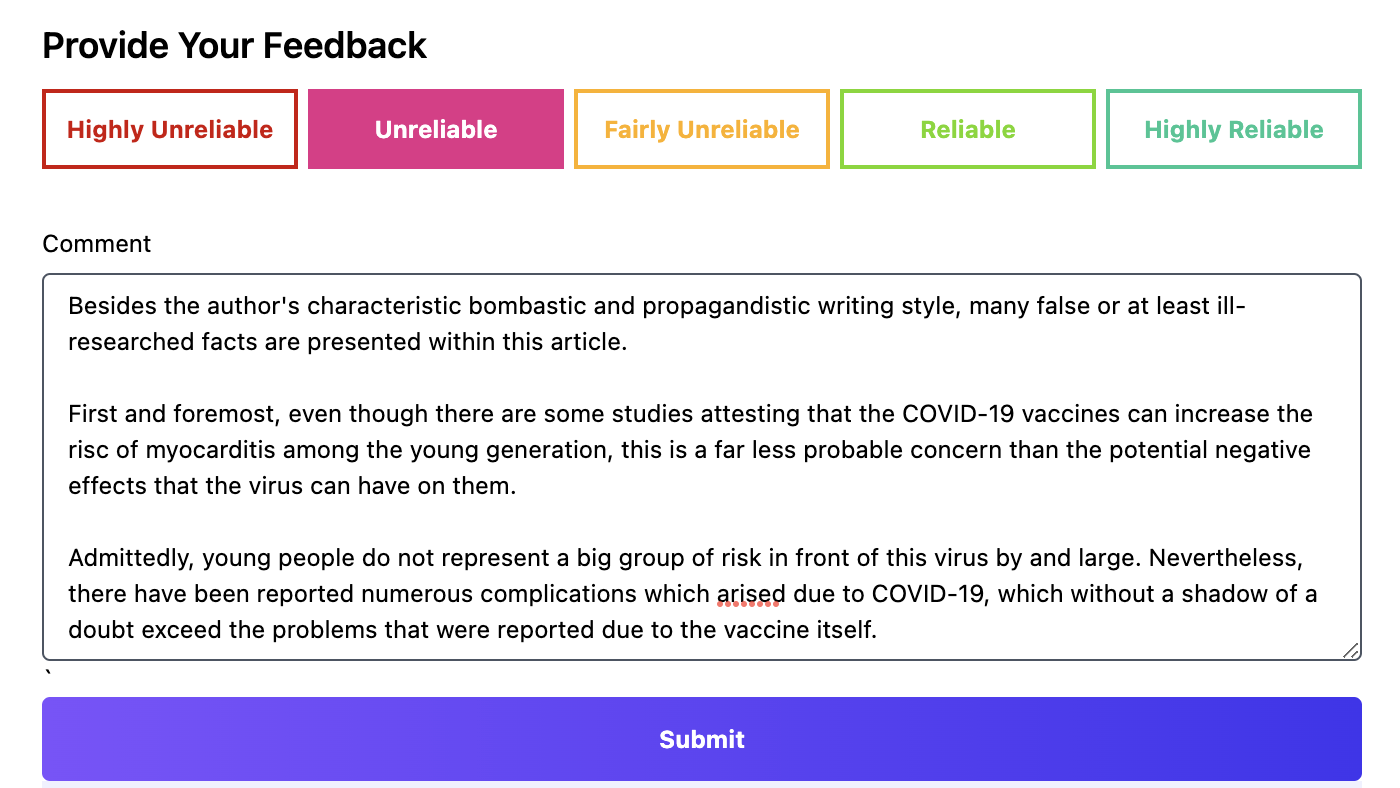
\includegraphics[width=0.9\textwidth,keepaspectratio]{images/user-feedack-form.png}}
  \caption{User feedback form screenshot from the application.}
\end{figure}